\chapter{System Design}
% -- C
\section{Creating Main Business Logic for Vertex}
\subsection{Models}
Vertex uses five models which are implemented from the Norton-API client-stubs. These stubs were generated from OpenAPI specification for the back-end python server, which has been aliased as Norton.
\\ The API stubs live in their own repository outside of the application. To use it in Flutter they are listed as a dependency in the projects 'pubspec.yaml' file.
\\ The business logic makes use of the models to pass data from the view-models to services.
See Figure~\ref{image:models}.

\begin{figure}[h!]
    \caption{Example of Models}
    \label{image:models}
    \centering
    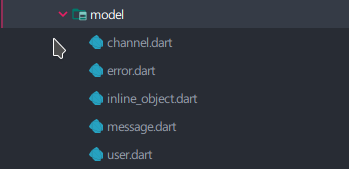
\includegraphics[width=0.7\textwidth]{images/models.png}
\end{figure}

\subsection{View Models}
A view model's purpose is to take data from a source and put it into a presentable form that the UI can interpret.
\\ Vertex uses four view-models to handle CRUD (Create, Read, Update, Delete) operations and update state. To understand how one works see figure~\ref{image:channelViewModel} for a breakdown of the class.

\begin{figure}[h!]
    \caption{Channel View Model Code Example}
    \label{image:channelViewModel}
    \centering
    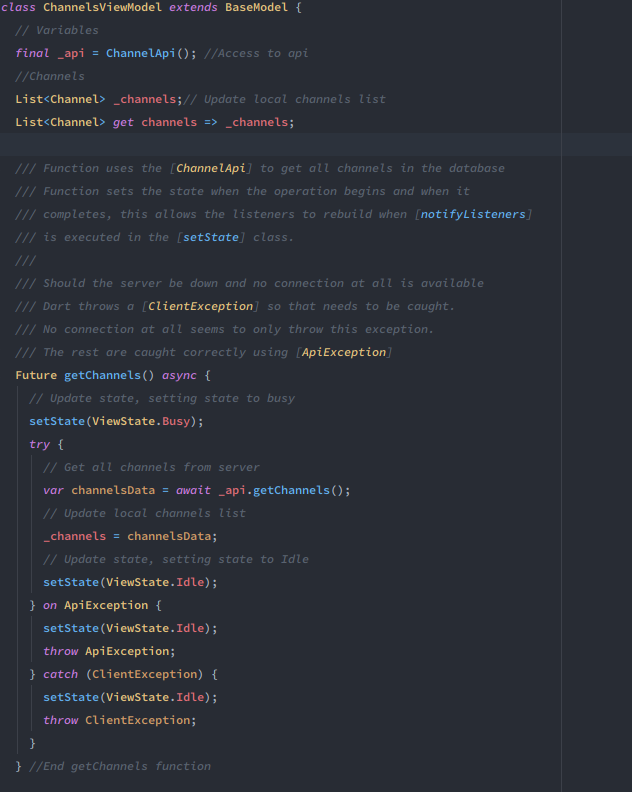
\includegraphics[width=1.0\textwidth]{images/channel_view_model_code.png}
\end{figure}

Figure~\ref{image:channelViewModel} is the ChannelViewModel class. As described in the comments it is the function that gets all the channel data from the server and updates the applications state.
\\\\ Note the following in figure~\ref{image:channelViewModel}: 
\begin{enumerate}
    \item The class is extending a class called BaseModel which is in charge using Change Notifier which provides ‘notifyListeners()’. This allows for widget rebuild.
    \item The API service is declared as \_api, this allows access to the Norton-API-client stubs CRUD functions for Channels.
    \item The Lists store a list of Channels using the Channels model locally so widgets can access its data.
    \item Inside the getChannels() setState() is classed passing ‘ViewState.Busy’, this notifies the listening widgets that an operation is taking place so the widget is able to display a progress indicator. 
    \begin{enumerate}
        \item The channel data is fetched from the server using the API-client stubs.
        \item The local List is updated with the channel data.
        \item setState() is called again setting its state to ‘ViewState.Idle’. This then notifies the listening widget to build with the new data received from the server.
    \end{enumerate}
    \item The final part looks after expectations thrown from the API-client stubs or Dart client exceptions. Should an exception be thrown the UI is updated to reflect the exception in an alert Dialog. 
\end{enumerate}
All other view models are built the same but just in charge or different data or views. In summary, the view models call setState() to update the UI with the new state. This pattern can be used with Streams in Flutter as well but for this application Future functions were used as they are asynchronous.

\subsection{Adding a Services Locator and Injecting Services}
The view-models are injected as a service into the application at run time with the help of a package called ‘get\_it’. \textit{“This is a simple Service Locator for Dart and Flutter projects with some additional goodies highly inspired by Splat. It can be used instead of InheritedWidget or Provider to access objects e.g. from your UI.”} [ADD ME: 1]. This allows for access to the view-models anywhere in the application by calling the locatorGlobal and the name of the service you wish to access. ‘get\_it’ is another dependency which is set in the applications pubspec file. 
\\ All services are registered as a Lazy Singleton, meaning it is created when it first gets invoked and it will always receive the same instance back. This is important as the view-models store data locally in Lists.
\begin{figure}[h!]
    \caption{Example of GetIt Class}
    \label{image:getItClass}
    \centering
    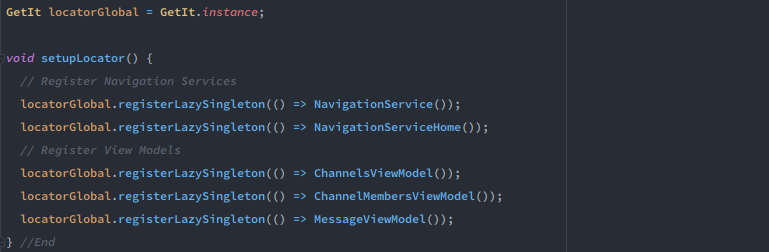
\includegraphics[width=1.0\textwidth]{images/get_it_class.png}
\end{figure}
\\\\Note the following in figure~\ref{image:getItClass}:
\begin{enumerate}
	\item Instance of ‘GetIt’ is created
	\item Navigation service View-models are registered
	\item In main.dart the main() function will call setupLocator() before calling runApp()
\end{enumerate}

\subsection{Implementing Provider}
Implementing Provider into the application is only a small part of the overall state management architecture implementation. Provider is another dependency that is listed in the applications pubspec.
\\ Provider has a widget called ChangeNotifierProvider. It is the widget that listens for changes in the view-model classes that extend ChangeNotify. With the use of ChangeNotify Provider and ChnageNotify in the application a widget/class called BaseView was created to aid in the process of fetching data and updating state. This class was adapted from a Flutter developers implementation of Provider and state management[ADD ME: 2]. Figure~\ref{image:baseViewClass} is a breakdown of the class.
\begin{figure}[h!]
    \caption{Example of BaseView Class}
    \label{image:baseViewClass}
    \centering
    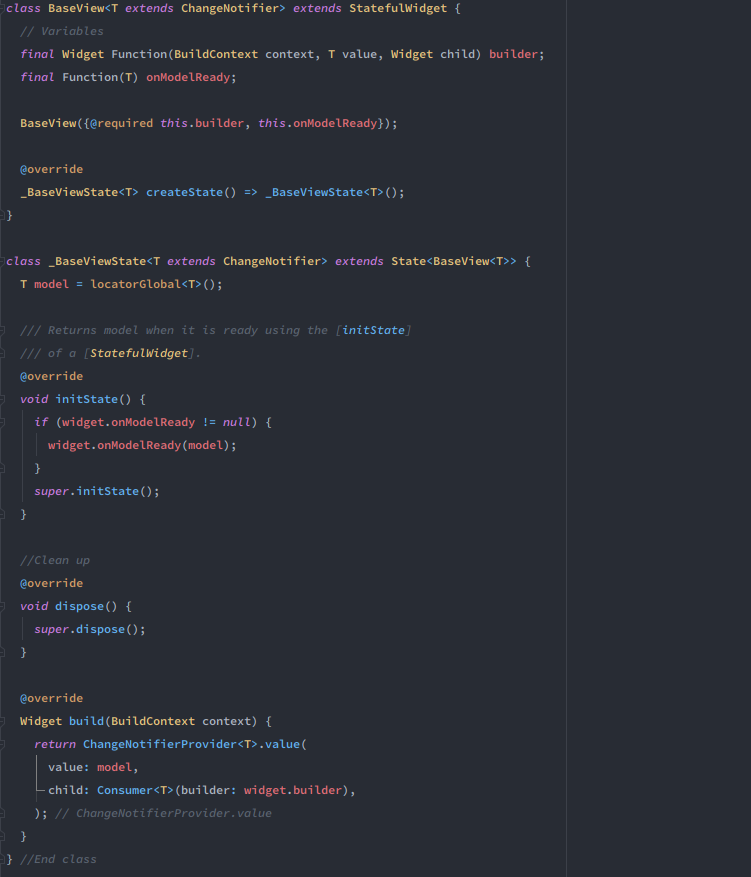
\includegraphics[width=1.0\textwidth]{images/base_view_class_code.png}
\end{figure}
\\\\Note the following in figure~\ref{image:baseViewClass}:
\begin{enumerate}
	\item The class converts a widget into a Stateful widget so the onInit function can be used to pass the model back to use in a callback function.
	\item Function(T) returns the model, this now gives access to the function inside that model class.
	\item The \textit{onModelReady} can now be used to notify the UI element that can display the data or display a progress bar depending on the BaseModel.state, the class that notifyListeners.
	\item The Widget Build function returns Providers ChangeNotifierProvider function with a value, the value being the view model and the child being the Consumer which has a build function. 
\end{enumerate}

\section{Integration With UI}
So with Provider and now the BaseView Widget it can all be put together in one of the view classes to retrieve data. Figure~\ref{image:messageViewBuilder} is a breakdown of how it works in the text chat view with message data:

\begin{figure}[h!]
    \caption{Example of MessageView Builder}
    \label{image:messageViewBuilder}
    \centering
    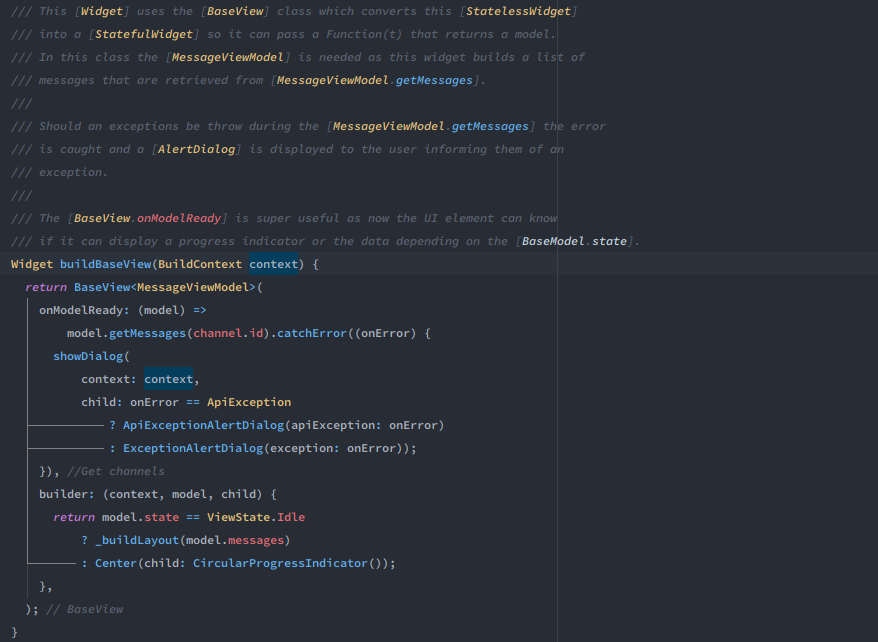
\includegraphics[width=1.0\textwidth]{images/messge_view_builder_with_model.png}
\end{figure}

Note the following in figure~\ref{image:messageViewBuilder}:
\begin{enumerate}
	\item Firstly the BaseView Widget is called passing it the view model that is needed, in this case, MessageViewModel.
	\item model.getMessages(channel.id) in the onModelReady calls the getMessages function from the view-model MessageViewModel. Should an error occur an exception dialog will be displayed to the user.
	\item The builder will return the \_buildLayout() Widget if the model.state is Idle else if will display a progress indicator until the model is ready.
	\item The \_buildLayout() now has the data needed to build its UI.
\end{enumerate}

\subsection{Handling State For WebRTC}
The state management is handled a little differently for WebRTC class due to a WebSocket being used to send and receive messages between the WebRTC signalling server. Voice and Video class handle state the same way just in different classes.
\\ When a user wishes to start a video call, the UI class creates an instance of the Signaling class, this class is in charge of connecting to the signalling server, gathering peer data, processing message events and setting up calls with peers when a peer is invited. See Figure~\ref{image:videoSignallingConnectFunc}.
\begin{figure}[h!]
    \caption{Example of Video and Signalling Connection Function}
    \label{image:videoSignallingConnectFunc}
    \centering
    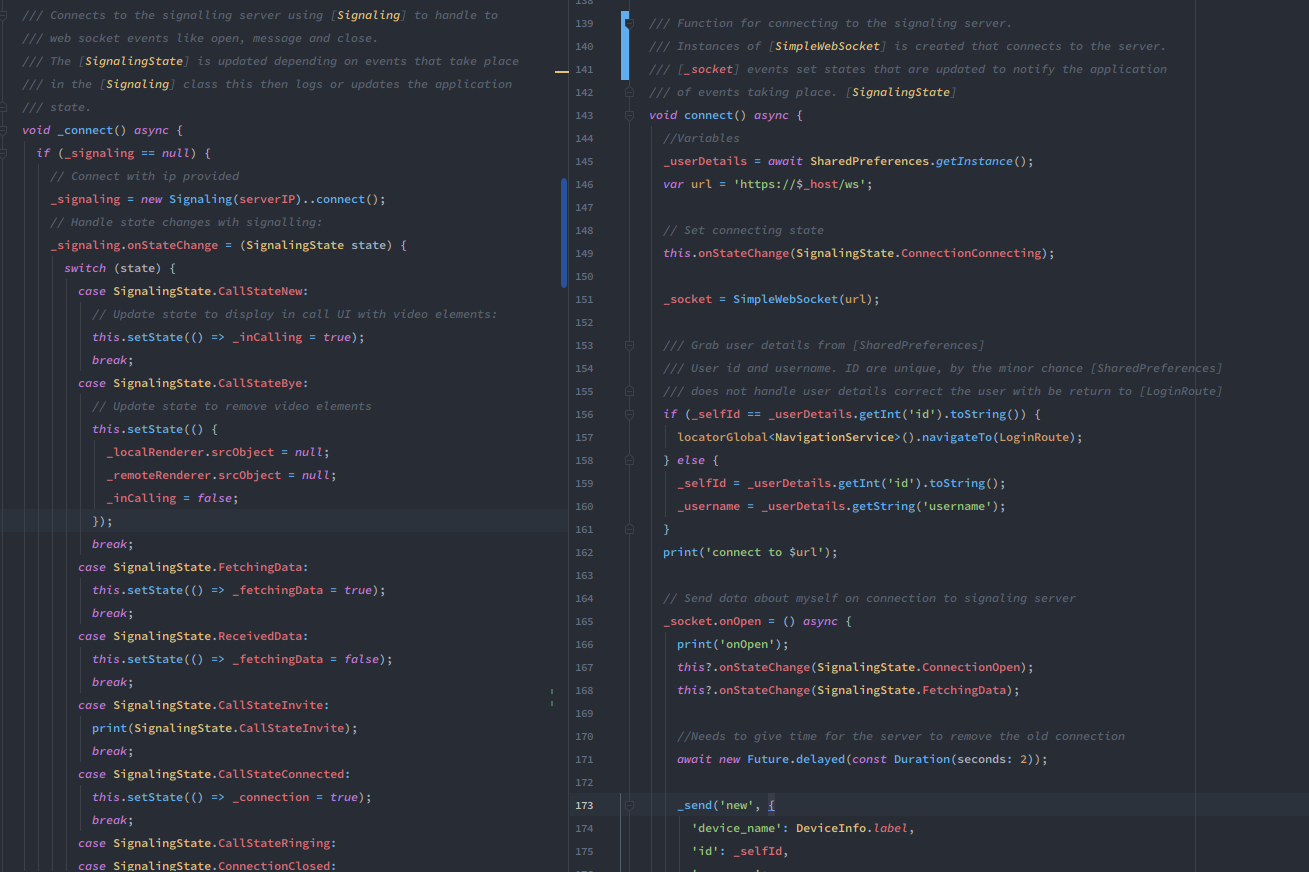
\includegraphics[width=1.0\textwidth]{images/video_and_signalling_connect_fcuntions.png}
\end{figure}

Note the following in figure~\ref{image:videoSignallingConnectFunc} on the left side:
\begin{enumerate}
	\item The Video UI class creates a new instance of the Signalling class passing it the server IP address.
	\item The Video UI class uses the callback function onStateChange declared in the Signalling class to listen for SignallingState changes. When an event is triggered in the Signalling class the Video UI state is updated depending on the SignallingState passed back in the callback function.
\end{enumerate}

Note the following in figure~\ref{image:videoSignallingConnectFunc} on the right side:
\begin{enumerate}
	\item The initial state is set to SignalingState.ConnectionConnecting, this Notifies the UI that the Signalling class is connecting to the WebRTC signalling server.
	\item An instance of SimpleWebSocket created passing it the URL to connect to the WebRTC signalling server.
    \item When the socket opens the connections to the server two new SignallingStates are set, \textit{SignalingState.ConnectionOpen} to notify of the connection successfully opened and \textit{SignallingState.FetchingData} to notify the UI its gathering data from the server, this allows the Video UI class to display a progress bar until the data is received back and the SignallingState is set to \textit{SignallingState.ReceivedData}. All messages that are received are processed accordingly and the appropriate state is set.
\end{enumerate}

% -- M
\section{Screen Shots}
Login Page See Figure~\ref{image:loginPage}
\begin{figure}[h!]
    \caption{Login Page}
    \label{image:loginPage}
    \centering
    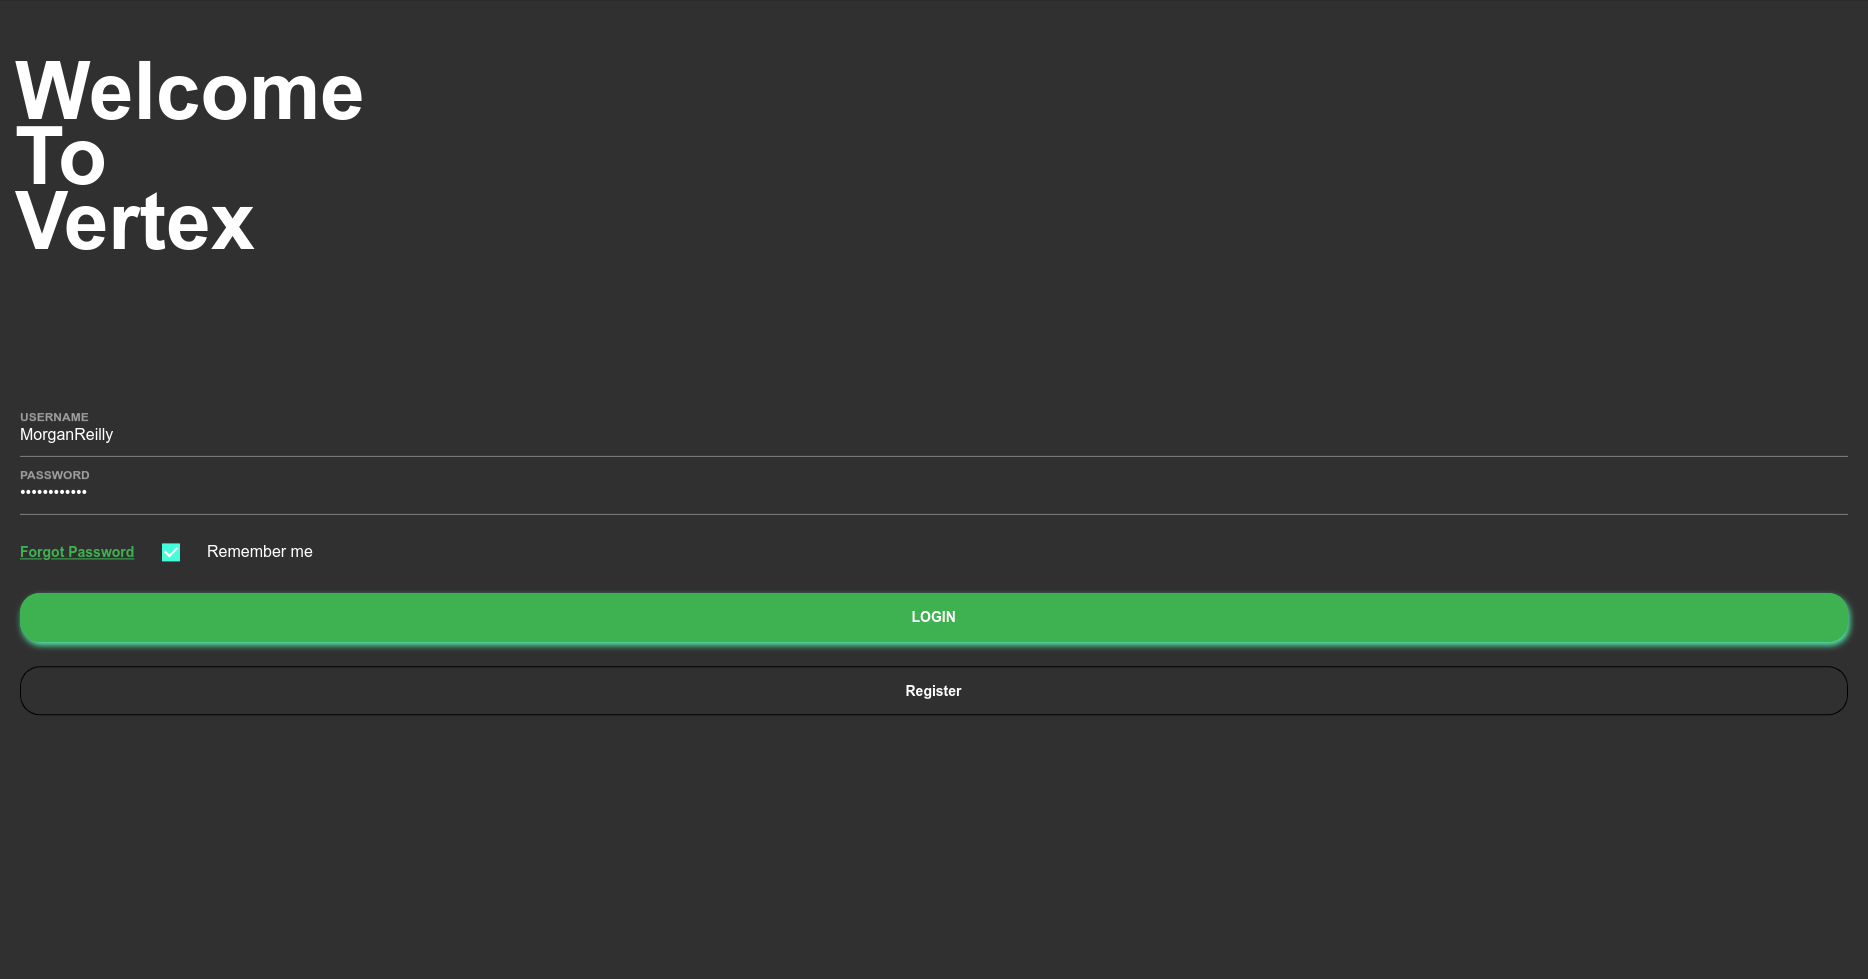
\includegraphics[width=0.7\textwidth]{images/pageScreenshots/loginPage.png}
\end{figure}

Register Page See Figure~\ref{image:registerPage}
\begin{figure}[h!]
    \caption{Register Page}
    \label{image:registerPage}
    \centering
    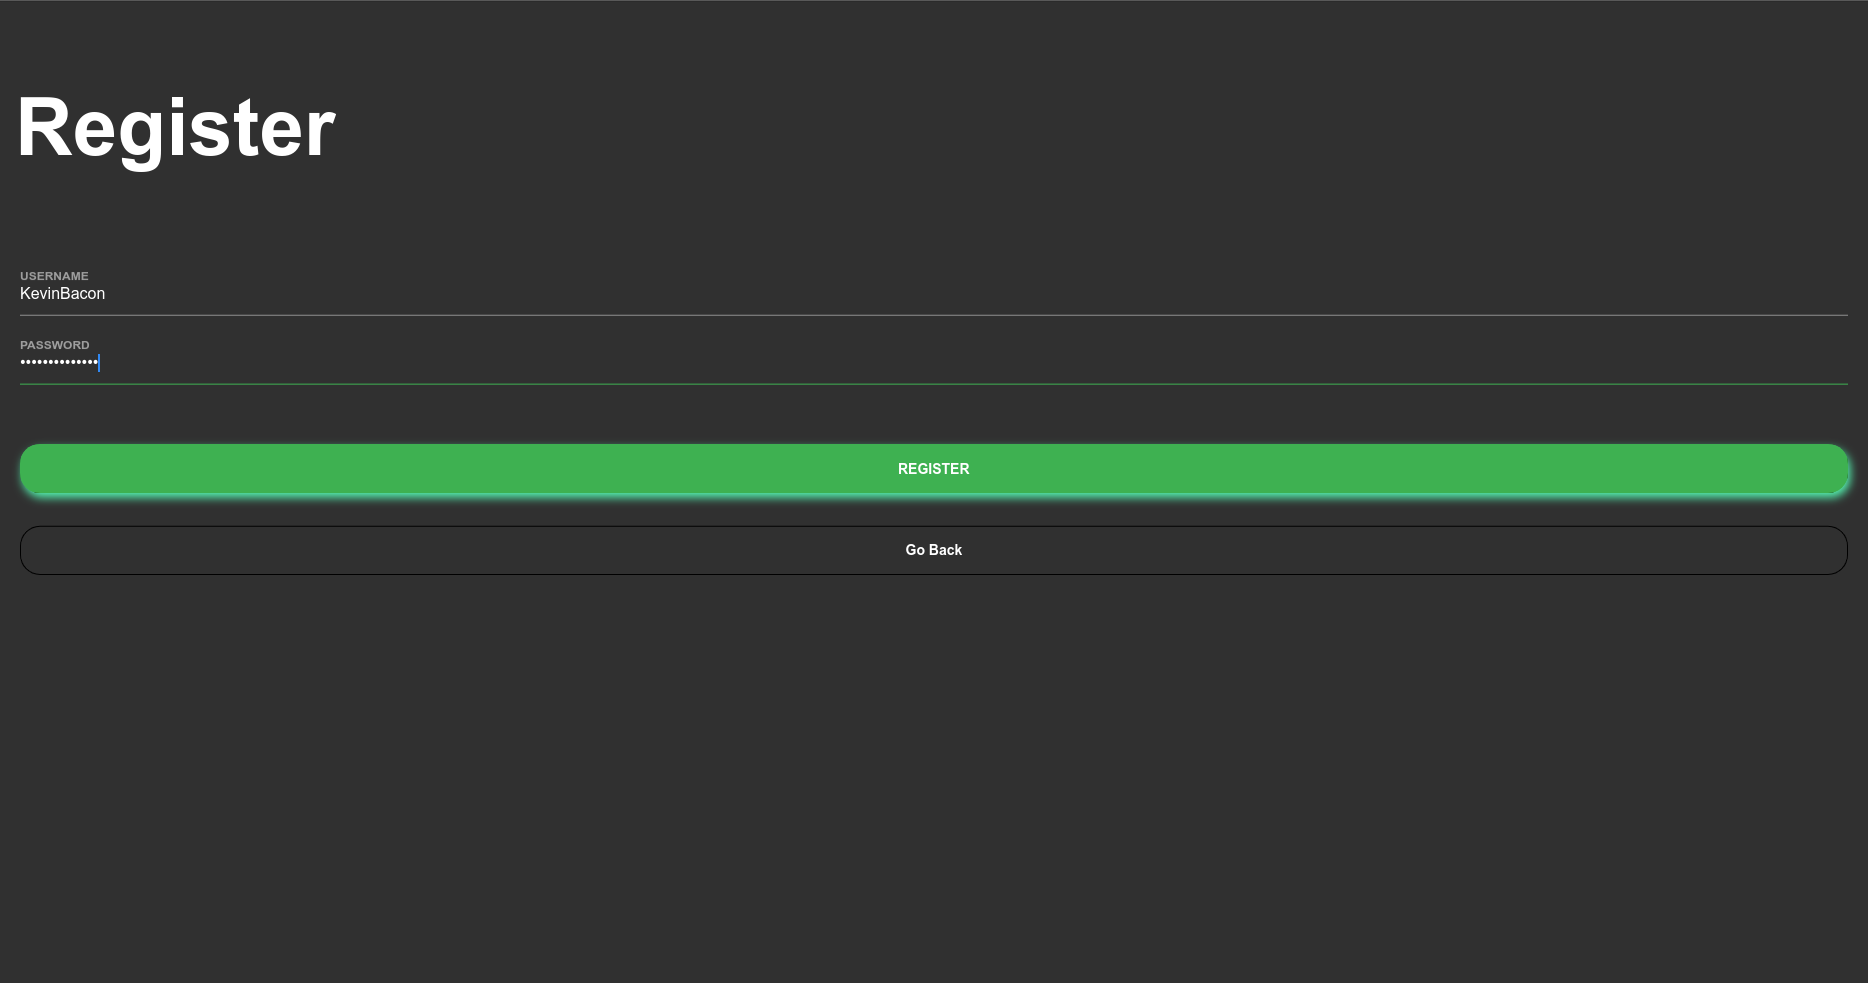
\includegraphics[width=0.7\textwidth]{images/pageScreenshots/registerPage.png}
\end{figure}

Home Page See Figure~\ref{image:homePage}
\begin{figure}[h!]
    \caption{Home Page}
    \label{image:homePage}
    \centering
    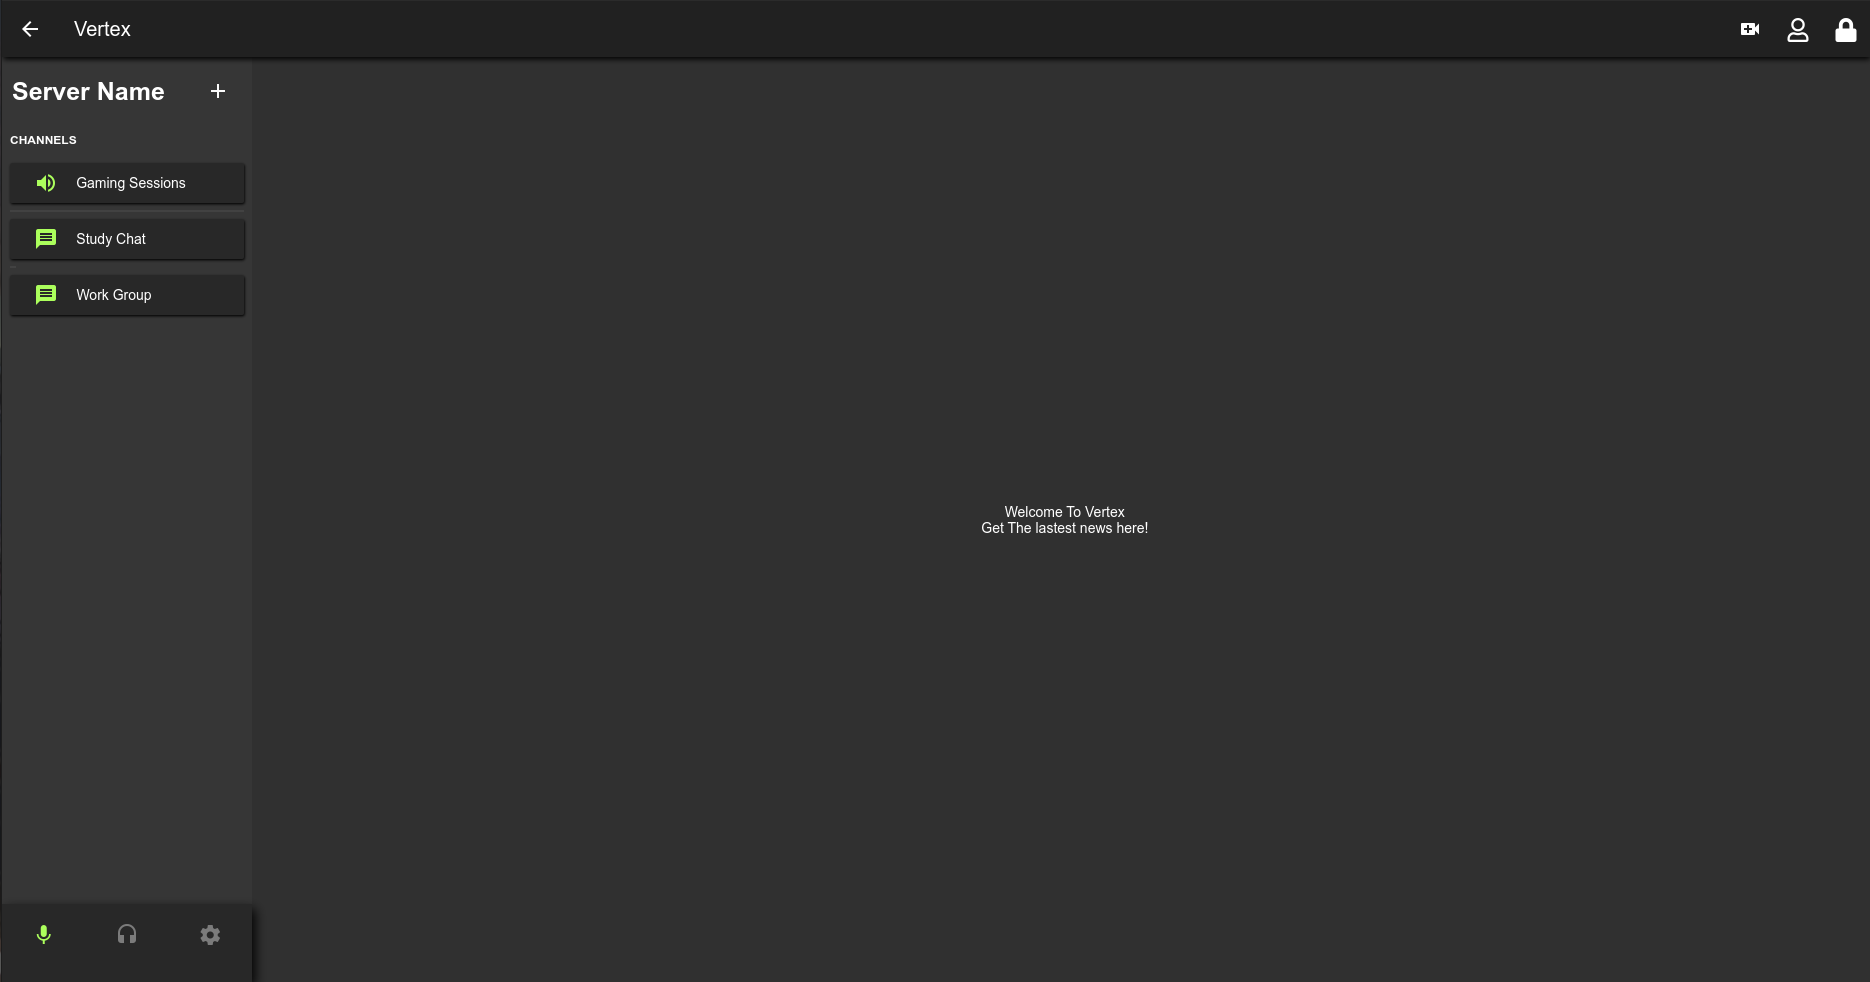
\includegraphics[width=0.7\textwidth]{images/pageScreenshots/homeScreen.png}
\end{figure}

Peer Connection Lobby See Figure~\ref{image:peerConnectionLobby}
\begin{figure}[h!]
    \caption{Peer Connection Lobby}
    \label{image:peerConnectionLobby}
    \centering
    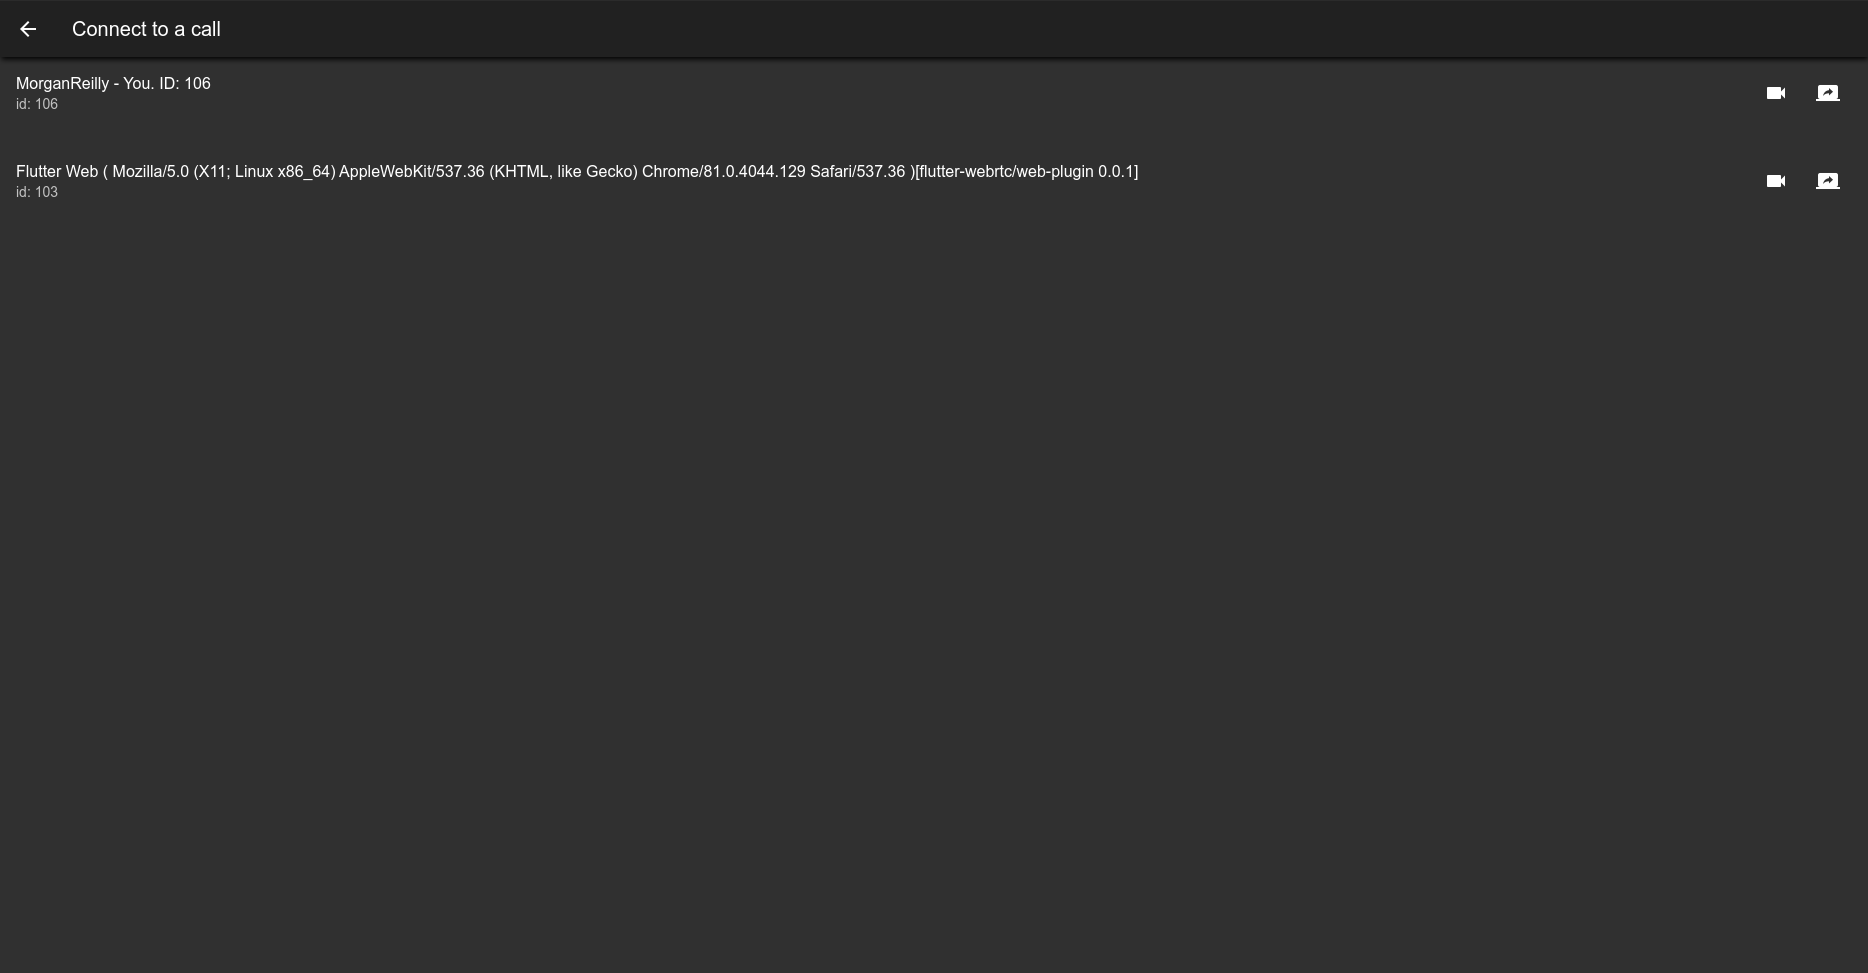
\includegraphics[width=0.7\textwidth]{images/pageScreenshots/callLobby.png}
\end{figure}

Successful WebRTC Functionality See Figure~\ref{image:webRTCProof}
\begin{figure}[h!]
    \caption{Successful WebRTC Functionality}
    \label{image:webRTCProof}
    \centering
    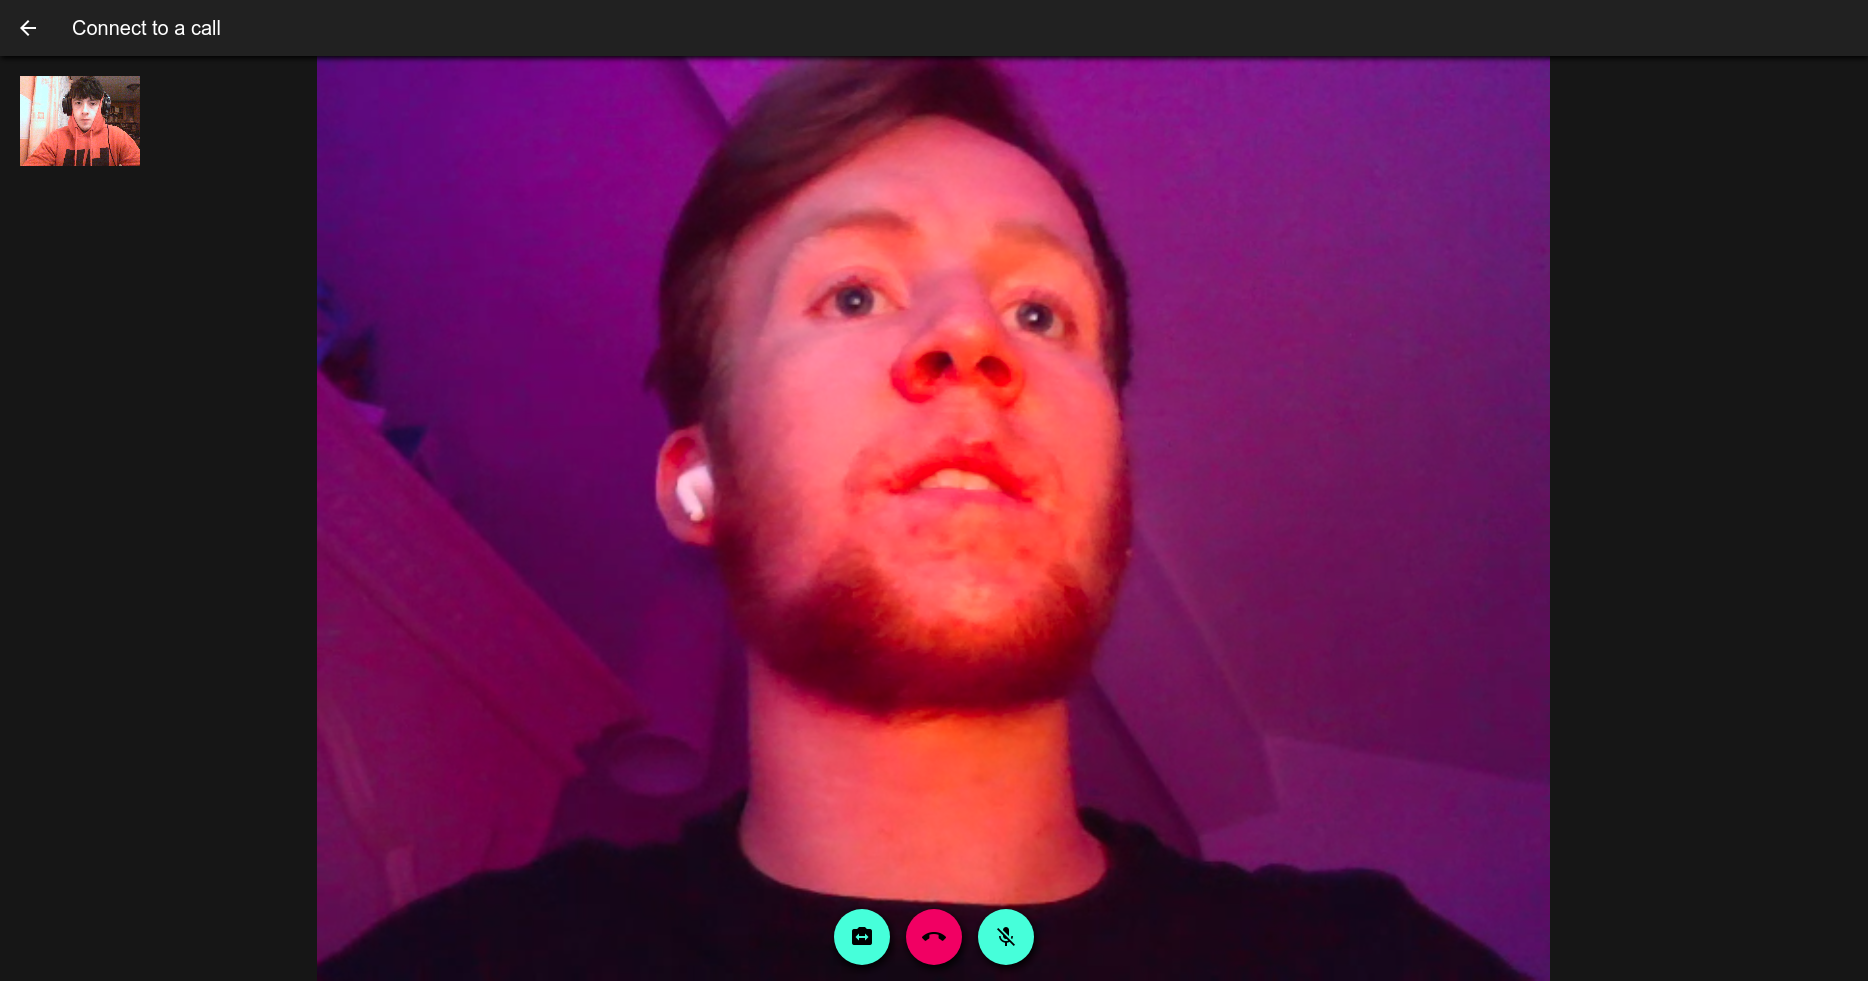
\includegraphics[width=0.7\textwidth]{images/pageScreenshots/webRTCProof.png}
\end{figure}

Channel Creation See Figure~\ref{image:channelCreation}
\begin{figure}[h!]
    \caption{Channel Creation}
    \label{image:channelCreation}
    \centering
    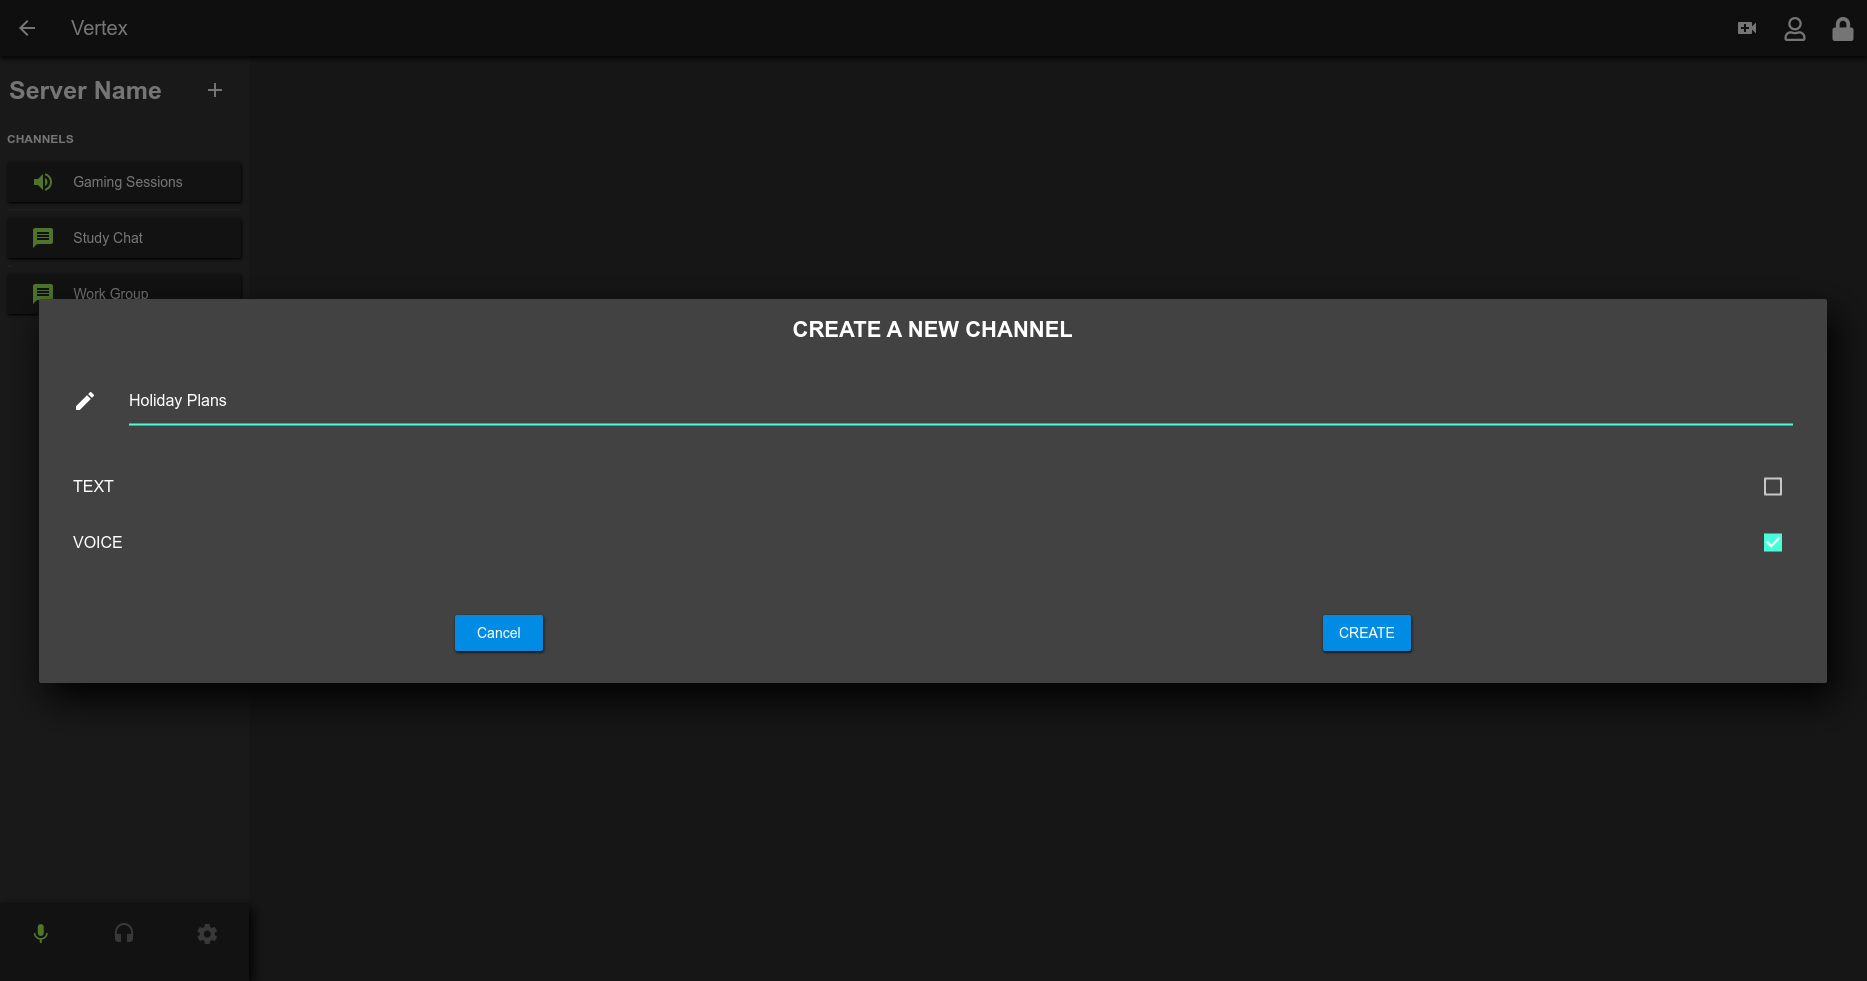
\includegraphics[width=0.7\textwidth]{images/pageScreenshots/channelCreation.png}
\end{figure}

Channel Deletion See Figure~\ref{image:channelDeletion}
\begin{figure}[h!]
    \caption{Channel Deletion}
    \label{image:channelDeletion}
    \centering
    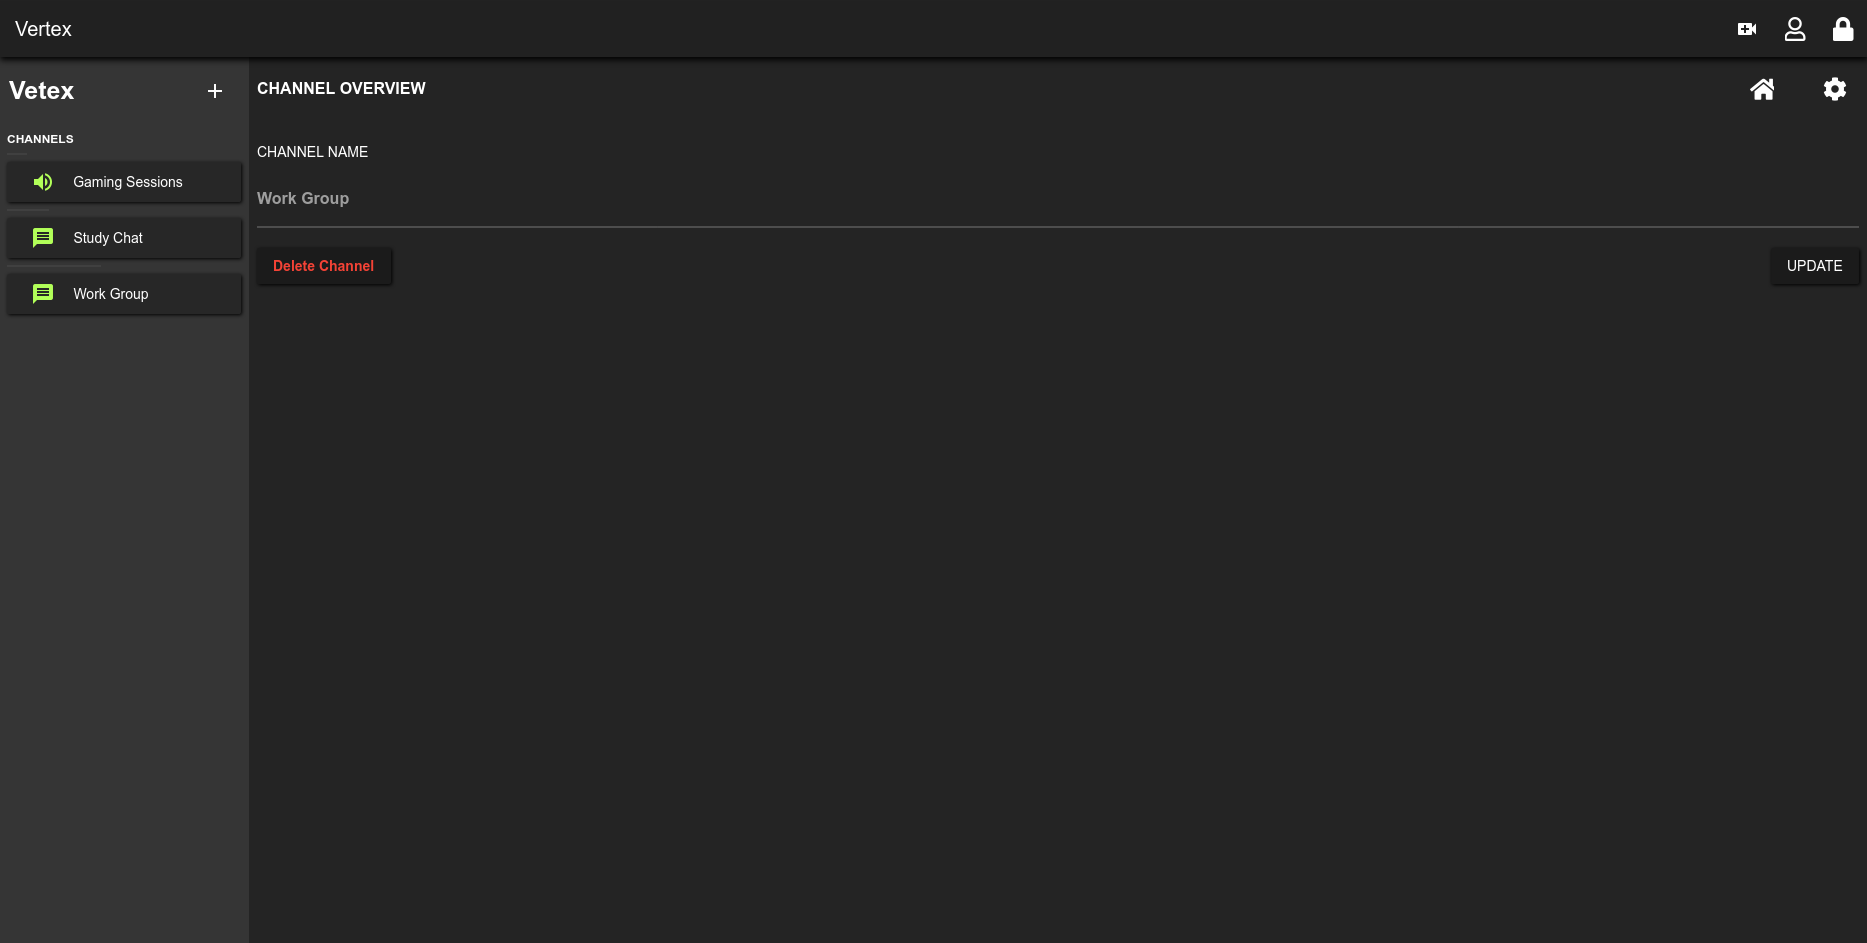
\includegraphics[width=0.7\textwidth]{images/pageScreenshots/channelDeletion.png}
\end{figure}

Settings Page See Figure~\ref{image:settingsPage}
\begin{figure}[h!]
    \caption{Settings Page}
    \label{image:settingsPage}
    \centering
    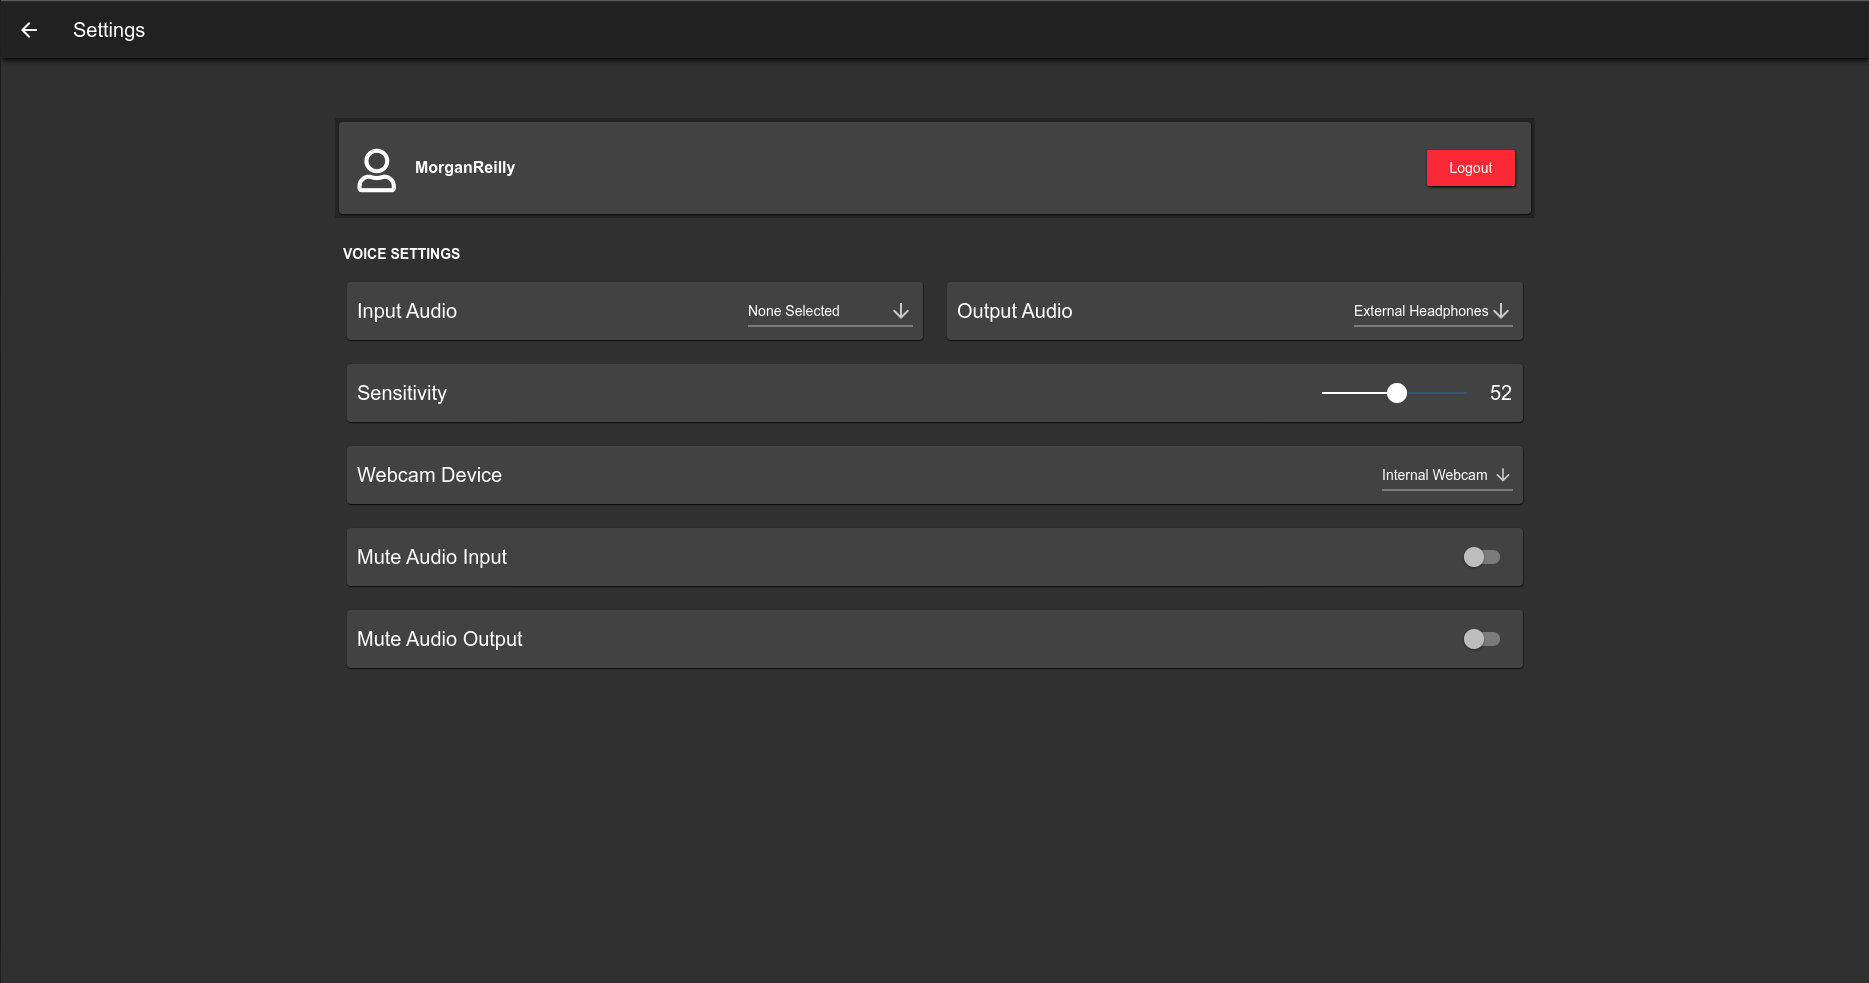
\includegraphics[width=0.7\textwidth]{images/pageScreenshots/settingsPage.png}
\end{figure}


\section{Database}
For vertex a MySQL was chosen as the application database. This was ultimately a big decision as the application could have used any assortment of SQL style databases, a noSQL database, or could have gone with a graph database, or possibly even a document store.
\\ This database uses an INNODB engine, which allows for full transaction support, various levels of locking, such as row-locking, and has full ACID compliance. The alternative which could have been used is a MYISAM engine, which supports different functionality which would not have suited the application.

\subsection{Schemas}
Due to the nature of the application only a handful of schemas were needed to handle the information saved throughout the application. The information being held is relatively straightforward. For each of the tables they need a unique identifier. In the case of schemas: User; Channel; Message; and Session; this was handled with the use of an auto-incrementing integer value, which increments by 1 per entry and starts at various values in respect to each table i.e. User will auto-increment from 100, Channel will auto-increment from 200 and so on. These auto-incrementing values are used in the form of the primary key for those tables with an alias of ‘id’ for each table allow for an ease of lookup, along with an O(1) time-complexity for look-up.
\\ The other remaining table, Member, uses foreign key values in a unique combination to handle look up, instead of a primary key value. For the most part, since there are few components of entry in each schema, the varaibles are given a ‘NOT NULL’ modifier, which means that data has to be given to them in order to avoid errors being raised.
\\ The database uses UTF-8 default as it’s character set, and utf8\_general\_ci as it’s collate set.
\\ The following schemas use cascading update, and cascading delete: Channel; Message; Session; Member. This allows for safe removal or modification of data, without setting null values.

\subsubsection{User Schema}
This schema handles the user information and was the first schema which had to be thought about.
\\ The User table is broken down into 3 components: ‘id’, ‘name’, ‘password’.
\\The ‘id’ of this table is described above, as an unsigned auto-incrementing integer starting at 100.
\\The ‘name’ is stored as a varchar of size 32 with a not-null modifier. This allows for an adequate size of allocated storage for the user name. The purpose of limiting the character is for memory preservation. The ‘name’ acts as a unique key to this schema. This is to avoid any duplication errors for any new users being inputted into the table, and also serves as a reference point should the ‘name’ need to be queried without explicitly knowing the ‘id’ beforehand. 
\\The ‘password’ is stored after it is hashed and salted using the bcrypt hashing function, which utilises the blowfish cipher. It is stored as a varchar of size 255 with a not null modifier.
See Figure~\ref{image:userSchema}

\subsubsection{Channel Schema}
This schema handles the channels being used in the application, and is broken down into 4 components.
\\The ‘id’ of this table is described above, as an unsigned auto-incrementing integer starting at 200.
The channel has to store a ‘name’ which forms part of a unique key used for referencing and duplication avoidance. This value is stored as a varchar of size 32 with a not null modifier.
\\It has a 'creator\_id', which acts as a foreign key from the User table (id).
\\It has a enumerated value, ‘type’, which allows us to differentiate between voice and text channels. This allows the user to create channels with a bit of variance to them.
\\Its unique key consists of ‘name’, ‘creator\_id’, and ‘type’ which serves as a way to avoid duplication's in the database.
See Figure~\ref{image:channelSchema}

\subsubsection{Message Schema}
This schema handles the messages being sent in the application. It is broken down into 5 components.
\\The first being the ‘id’. This is an unsigned auto-incrementing integer starting at 300.
\\The second being ‘channel’, which is a foreign key relating to the Channel table (see Channel for details). This serves as a way to link the message to the channel, without the messages spilling out into incorrect channels.
\\The third component is the ‘author’, which is a foreign key relating to the User table (see User for details). It serves as a way to link the message to the relevant user, without incorrect users seeing the data.
The fourth component is ‘content’. This is a varchar of size 255 with a not null modifier. This variable stores the message content that the user is sending.
\\The final component of this schema is the ‘timestamp’ for the message. This is stored as an Int of size 8 with a not null modifier.  The timestamp is stored as Unix Epoch time and the purpose of the size being set to 8 for this is to allocate enough space to handle epoch time correctly.
See Figure~\ref{image:messageSchema}

\subsubsection{Session Schema}
This schema handles the current session that is active for the user. It is a fairly straight-forward schema which consists of 3 components.
\\ The first component is the ‘id’. This is a varchar of size 255 with a not null modifier. The reason being is that the id should be stored as a UUID, therefore requiring an adequate amount of space allocation for the variable. This is the primary key for this table.
\\ The second component is ‘user’. This is a foreign key which links this table to the User table (see User for details).
The final component is ‘expire\_after’. This is another instance of Unix Epoch time, with a similar allocation of memory for this variable as was seen in the Message table. 
See Figure~\ref{image:sessionSchema}

\subsubsection{Member Schema}
The final table in this database is the Member table. This is responsible for grouping users with relevant channels, which allows for easier look-ups. It consists of 2 components, both of which are foreign keys.
\\ The first component is ‘channel’. This is set as an Integer of size 4, and is a  foreign key which relates to the Channel table on ‘id’.
\\ The second, and final component, is the ‘user’. This is also set as an Integer of size 4, and is a foreign key which relates to the User table on ‘id’.
\\ This table contains a unique key, which is comprised of  ‘channel’ and ‘user’. The reason being is to avoid duplicate entries in this schema, and also helps with look ups on the table.
See Figure~\ref{image:memberSchema}

\subsection{Testing}
In terms of testing, a full CRUD test is included in ‘vertex\_db\_v2.sql’, which is located on the database portion of the project repository. These tests verify correct functionality of creation of values, reading values, updating values, and deletion of values. They also verify and test for referential integrity for the database, along with duplication avoidance.

\begin{figure}[h!]
    \caption{User Schema}
    \label{image:userSchema}
    \centering
    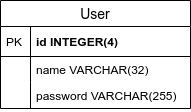
\includegraphics[width=0.3\textwidth]{images/UserSchema.png}
\end{figure}

\begin{figure}[h!]
    \caption{Channel Schema}
    \label{image:channelSchema}
    \centering
    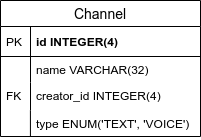
\includegraphics[width=0.3\textwidth]{images/ChannelSchema.png}
\end{figure}

\begin{figure}[h!]
    \caption{Message Schema}
    \label{image:messageSchema}
    \centering
    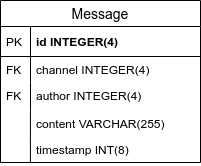
\includegraphics[width=0.3\textwidth]{images/MessageSchema.png}
\end{figure}

\begin{figure}[h!]
    \caption{Session Schema}
    \label{image:sessionSchema}
    \centering
    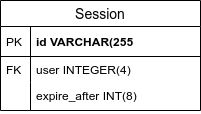
\includegraphics[width=0.3\textwidth]{images/SessionSchema.png}
\end{figure}

\begin{figure}[h!]
    \caption{Member Schema}
    \label{image:memberSchema}
    \centering
    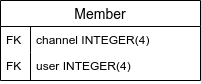
\includegraphics[width=0.3\textwidth]{images/MemberSchema.png}
\end{figure}

\begin{figure}[h!]
    \caption{Database Schema}
    \label{image:databaseSchema}
    \centering
    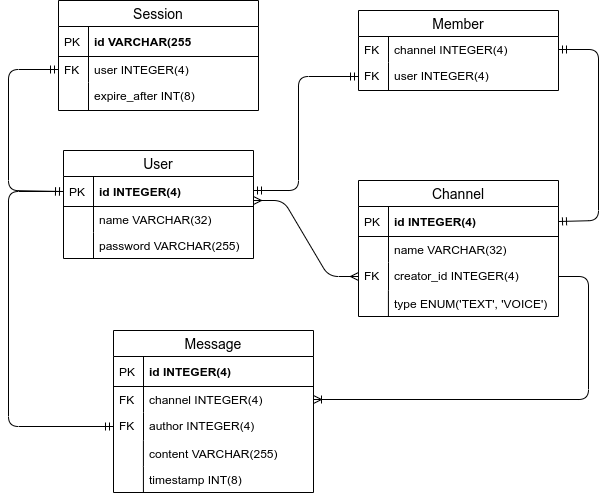
\includegraphics[width=1\textwidth]{images/FullSchemaDesign.png}
\end{figure}